\chapter{Gravity Inversion}\label{Chp:cook:gravity inversion}

\section{Introduction}

In this part the documentation we give an introduction on how to us the \downunder module using the 
inversion driver functions to perform the inversion of gravity and magnetic data. The driver functions 
enables geologists and geophysicists apply the \downunder module quickly and in easy way
with out a detailed knowledge of the theory of inversion or programming skills. However, users
how are interested in specializing or extending the inversion capacity are referred to the second part~\ref{part2}
of this manual. It is beyond the intention of this manual to give a in-detailed introduction to
geophysical inversion in particular to the appropriate preprocessing of data sets. We refer to~\cite{REF1, REF2, REF3}.


The \downunder function described here are designed for calculate estimations for the 
3-D distribution of density and/or susceptibility from 2-D gravity and magnetic data measured in ground 
or airborne surveys. This process is generally called inversion of geophysical data.
Following the standard assumption it is assumed that the 
data are measured as perturbation of an expected gravity and/or magnetic
field of the Earth. In this context measured gravity and magnetic data are in fact describing anomalies in 
gravity and magnetic field. As a consequence the inversion process 
provides corrections to an average density (typically $2670 kg/m^3$) and susceptibility (typically $0$). 
So in the following we will always assume that given data for anomalies are given and therefore
not in all cases explicitly use the terms such gravity anomalies or density corrections but just use the terms
gravity and density.

In this chapter we will give a detailed introduction into usage of the driver functions 
for inversion of gravity data. In the following chapters~\ref{Chp:cook:magnetic inversion} and~\ref{Chp:cook:joint inversion}
we will discuss the inversion of magnetic and the joint inversion of gravity and magnetic data using 
\downunder. As the same principles as for gravity data apply the presentation for these problem classes is kept short and 
users interested in magnetic data only should still work through this chapter on gravity data. 

To run the examples discussed you need to have \escript (version 3.3.1 or newer) installed on your computer.
Moreover, if you want to visualize result, you must have access to plotting software which is able to process
\VTK input files, e.g. \mayavi and \VisIt. As \mayavi can easily be obtained and installed for most platforms
the tutorial is based on \mayavi as visualization. However, it pointed out 
that \VisIt is the preferred visualization tool for \escript as it can deal with very large data sets more effectively.
    


\begin{figure}
\centering
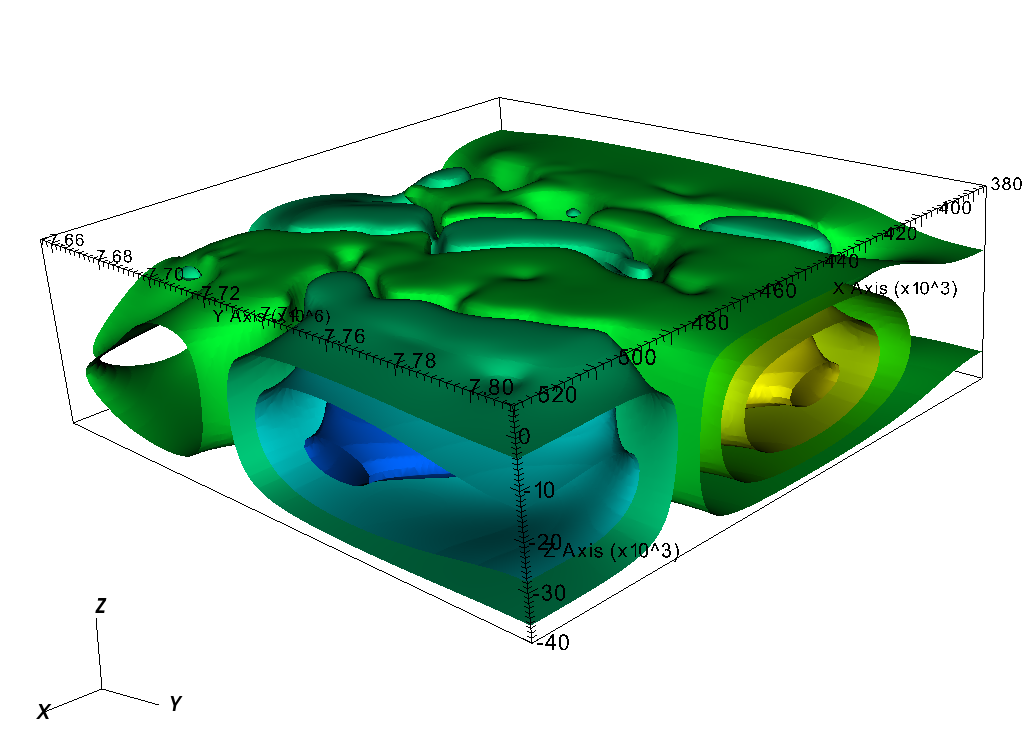
\includegraphics[width=\textwidth]{density10.png}
\caption{3D contour plot of density distribution of inversion of data \file{bouguer_anomaly.nc}. Colors
represent values of density where high values are represented by red and low values are represented by blue.}
\label{FIG:P1:GRAV:1}
\end{figure}

\section{How does it work?}
The execution of the inversion is controlled by script which is in essence is a text file. This can be edited using any 
text editor. The script contains a serious of statements which are executed from an interpreter which
is an executable program reading the text file and executing the statements line-by-line. In the case 
of \downunder the interpreter is \python. In order to be able to process the statements in each line of the script
certain rules (called syntax) need to be obeyed. There is large number of online tutorials for \python 
available\footnote{e.g. \url{http://www.tutorialspoint.com/python} and \url{http://doc.pyschools.com}}. We also 
refer to the \escript cook book \cite{ESCRIPTCOOKBOOK} and users guide \cite{ESCRIPT} which is in particular useful for users which who to dive deeper
\downunder. For this part of the manual no \python knowledge is required but it is recommended that 
users acquire some basic knowledge on \python as they progressing in their work with \downunder.

The following script~\ref{code: garvity1}\footnote{The script is similar to the \examplefile{gravity_netcdf.py} script
find in the \escript example file directory.} is a simple example to run an inversion for gravity data: 
\begin{pyc}
\
\begin{verbatim*}
# Header:
from esys.downunder import *
from esys.weipa import *
import esys.escript.unitsSI as U

# Step 1: set up domain
dom=DomainBuilder()
dom.setVerticalExtents(depth= 40.*U.km, air_layer=6.*U.km, num_cells=25)
dom.setFractionalPadding(pad_x=0.2, pad_y=0.2)
dom.fixDensityBelow(depth= 40. * U.km)

# Step 2: read gravity data
source0=NetCdfData(NetCdfData.GRAVITY, 'bouguer_anomaly.nc',altitude=0.)
dom.addSource(source0)

# Step 3: set up inversion
inv=GravityInversion()
inv.setSolverTolerance(1e-4)
inv.setSolverMaxIterations(50)
inv.setup(dom)

# Step 4: run inversion 
inv.getCostFunction().setTradeOffFactorsModels(10.) 
rho = inv.run()

# Step 5: write reconstructed density to file
saveVTK("result.vtk", density=rho)
\end{verbatim*}\label{code: garvity1}
\end{pyc}
The result, in this
case the density distribution, is written to an internal file for further processing. You can copy and past the text of the 
script into a file of any name, let's say for further reference we use the file name \file{grav.py}. It is recommendable
to use the extention \file{py} to identify the file as \python script. We will discuss the statements
of the script later in this chapter. 

Obviously the inversion needs to be fed with some gravity data. In this case 
the data are loaded from the file \file{bouguer_anomaly.nc} which available in the \escript example file directory. The data are given 
in the \netcdf data format for gridded data. After you have copied this file into the directory in which you have
saved the script \file{grav.py} you can run the program using the command line 
\begin{verbatim}
run-escript grav.py
\end{verbatim}
We are running \file{grav.py} through the \escript start-up command as \escript is used as a back end for the inversion 
algorithm\footnote{Please see the \escript users guide~\cite{ESCRIPT} on how to run 
your script in parallel using threading and/or MPI.}. Obviously it is  assumed that you have an
installation of \escript available on your computer, see \url{https://launchpad.net/escript-finley}.

After the execution has successfully been completed you will find the result file \file{result.vtk} in the directory
from where you have started the execution of the script. the file is using the \VTK format and can be important 
easily into many visualization tools. One option is the \mayavi package which is available on most platforms. You can invoke the
the visualization using the commands
\begin{verbatim}
mayavi2 -d result.vtu -m SurfaceMap
\end{verbatim}
from the command line. Figure~\ref{FIG:P1:GRAV:1} shows the result using contour plotting\footnote{Plots
have been created with \VisIt.}.

Let us have a closer look at the script\footnote{In \python lines starting with `\#` are commends and are not processed further.}: Besides the header section one can separate the script into five steps:
\begin{enumerate}
 \item set up domain on which the inversion problem is solved
 \item load the data 
\item set-up the inversion problem
\item run the inversion
\item further processing of the result, here we write the reconstructed density distribution to a file.
\end{enumerate}
In the following we will discuss the steps of the scripts in more details. Before we do this it is pointed out that
the header section which, by following \python standards, makes all the package we need available to access within the script. At this
point we will not discuss this in more details but emphasize that the header section is a vital part of the script. It is is required 
in each \downunder inversion script and should not be altered accept if additional modules are needed. 

\begin{figure}
\centering
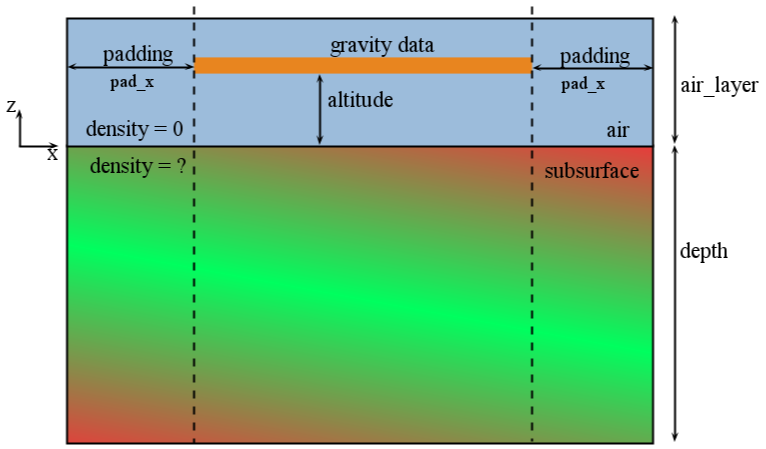
\includegraphics[width=\textwidth]{dom2D.png}
\caption{2D domain set-up for gravity inversion.}
\label{FIG:P1:GRAV:2}
\end{figure}

\section{How to create the inversion Domain}
First step in the script~\ref{code: garvity1} is the definition of the domain over which the inversion is performed.
We think of the domain as a block with orthogonal, plain faces. Figure~\ref{FIG:P1:GRAV:2} shows the set-up for 
a two dimensional domain (see also Figure~\ref{fig:domainBuilder} for 3D). The lateral coordinates along the 
surface of the Earth are denoted by $x$ and $y$ (on $x$-direction is shown). The $z$ direction defines the
vertical direction where the part above the surface has positive coordinates and the 
subsurface negative coordinates. The height of the section above the surface which is assumed to be filled to with air 
needs to be set by the user. The inversion assumes that the density in the section is known to be zero. The density
below the surface is unknown and is calculated through the inversion. The user needs to specify the depth below
the surface in which the density is to be calculated. 
The lateral extension of the domain is defined by the data sets fed into the inversion. It is chosen large enough
to cover all data sets. In order to reduce the impact of boundary a padding zone around the data sets can be introduced.
  
\begin{figure}
\centering
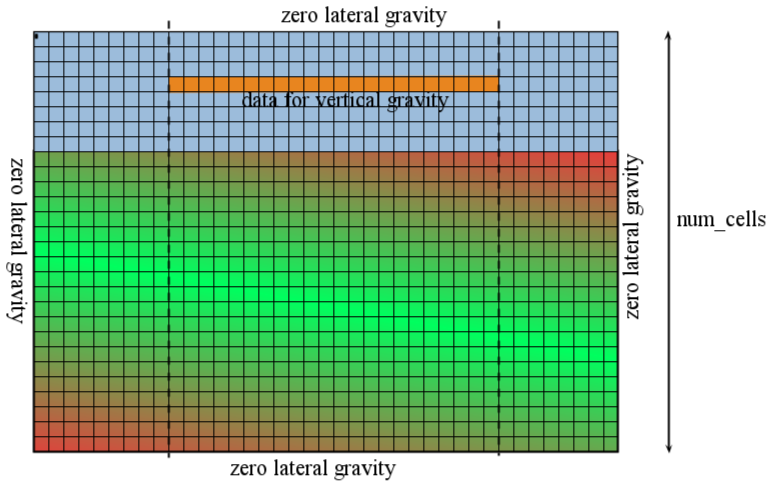
\includegraphics[width=\textwidth]{dom2DFEM.png}
\caption{Cell distribution and boundary conditions for 2D domain.}
\label{FIG:P1:GRAV:2}
\end{figure}

The reconstruction of the gravity field from an estimated density distribution is a the key component of the inversion process.
To do this \downunder uses the finite element method (FEM) to do this. We need to introduce a grid over the domain, see Figure~\ref{FIG:P1:GRAV:2}.
The number of vertical cells is set by the user while the number of vertical cells is derived from the grid spacing of the 
gravity data set(s). It is assumed that gravity field data given are constant across a cell. 
To be able to reconstruct the gravity field some assumptions on the values of the gravity field on the domain boundary
have to made. \downunder assumes that on all faces the lateral gravity field component equals 
zero. No assumptions on the 
horizontal components are made\footnote{It is assumed that the gravity potential equals zero on the top and bottom
surface, see Section~\ref{sec:forward gravity} for details}\footnote{Most inversion codes are using Green's function over an unbounded domain to reconstruct the gravity field. This approach
makes the assumption the gravity field (or potential) is converging to zero when moving away from the region of interest. The 
boundary conditions used here are stronger in the sense that the lateral gravity component is enforced to zero in 
a defined distance of the region of interest but weaker in the sense that no constraint on the horizontal component is applied.}.
   
In script~\ref{code: garvity1} the statement
\begin{verbatim}
dom=DomainBuilder()
\end{verbatim}
creates same form of a factory to build a domain. 
We define the features of the domain we would like to create:
\begin{verbatim}
dom.setVerticalExtents(depth= 40.*U.km, air_layer=6.*U.km, num_cells=25)
dom.setFractionalPadding(pad_x=0.2, pad_y=0.2)
\end{verbatim}
Here we define the depth of the domain to $40 km$, the thickness of the air layer above the surface to $6km$ and 
the number of vertical cells to $25$. We also introduce a lateral padding of $20 \%$ of the expansion of
the gravity data on each side of the data and in both lateral directions.

In some cases it can be appropriate to assume that the density below a certain depth is 
zero\footnote{As we are in fact calculate density corrections this means that the density is assumed to be
the average density.}. The statement 
\begin{verbatim}
dom.fixDensityBelow(depth= 40. * U.km)
\end{verbatim}
introduces this constrain. As in the case discussed here the depth for zero density is not less than the
depth of the domain no constraint at depth is applied to the density.

ADD U 

\section{Getting the Data in}

\section{Set-up Inversion and run the show}

\section{Take a look}

\section{Remarks}

=====


Before we do this a few words about the header section of the script:
\begin{verbatim*}
from esys.downunder import *
from esys.weipa import *
import esys.escript.unitsSI as U
\end{verbatim*}
The \verb|import| statement makes certain functions directly available for usage in the script. After \downunder
has been imported in the first import statement all functions in the \downunder package cane directly been used,
eg. we can call \verb|DomainBuilder| to create a domain for the inversion. Similar 
the second import statement makes all the \weipa functions ready for usage in the script. 
Here we will in particular use the \verb|saveVTK| function to write the inversion result to 
an external file\footnote{See also \escript users guide~\cite{ESCRIPT}.}.


For instance we can
directly call which is part  Here we 
load all the functions of \downunder which is the inversion tool kit and \weipa which supports the output 
of the inversion into various file formats. Notice that both package use \escript so this is also imported behind the scenes.
The third \verb|import| statement makes the 
$40 km$
\verb|40 * U.km| 
 

 

 

==============================

will not make a difference between gravity and gravity anomalies 
and density and density corrections. We will loosely use the terms density and gravity when referring to corrections and anomalies.  

When using \downunder driver function it is also assumed that the necessary corrections (e.g. for height and topography) are applied 
before data are fed into the inversion. 
 
To solve the inversion problem 
the earth is modeled using a large number of points - so called nodes - in a rectangular grid.
Density and susceptibility are estimated on these nodes. 
There distribution is obtained by minimizing a cost function to fit the observed data and to achieve 
a desirable smoothness of the distribution of density and susceptibility. 

 

Density and susceptibility as well as the resulting gravity and magnetic field
are calculated as a distribution across a hexahedron which contains a subsurface region of the Earth filled
with solid material of unknown density and susceptibility and a surface area filled with air 
in which the gravity and magnetic field are measured and density and susceptibility are in fact known.

The inversion problem is solved in an iterative manner 
where an estimation of the density and susceptibility distribution
is improved through a series of update steps in order to fit the result with the input data. 
This iteration process is terminated after a stopping criteria is met, e.g. when the estimated 
termination error reaches a given tolerance.





\begin{figure}
\centering
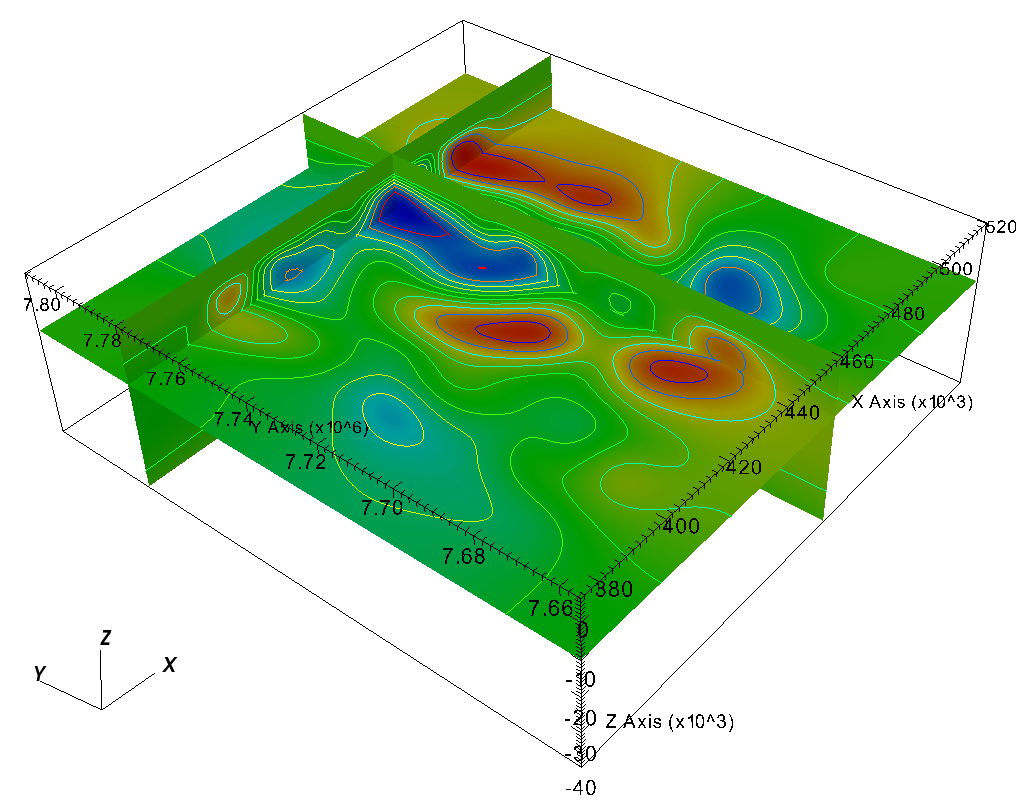
\includegraphics[width=\textwidth]{density11.png}
\caption{Depth image across previous 3D gravity inversion which presents discrepancy in density. Diversity in density are detected with colors and contours.}
\end{figure}





\section{Gravity Data}
Theoretically weighs depends on the force of gravity at 
that position and the force of gravity varies with elevation, rock densities, latitude and topography. 
Mass, however, does not depend on gravity but is a constitutive quantity throughout the earth. So the
spring stretch in mass suspension is related to the gravity force. In addition with a constant mass, 
difference in spring stretch illustrate the changes in acceleration of gravity. The principal of gravity exploration 
is based on the topography of the basement, thickness of the sedimentary section with various density, porosity of 
the layer and elevation.

The amount of $g$ at sea level is about 980 $kg/s^2$ or 980,000 $mgal$. Gravity acceleration 
is measured in two types. The first corresponds to specify the absolute magnitude of gravity 
at any place and the second refers to the alteration in gravity from one place to another. 
In gravity study variation of this value which is caused by underground structure, is plotted as a residual gravity.
Closed variation in residual gravity indicates discrepancy in subsurface geological structure.

The Gravity data are taken from onshore and offshore observation recorded at many gravity stations with high precision 
of determination in elevation and position (latitude and longitude). All raw reading gravity observations require 
to process with many corrections.

The sun and moon gravitational forces make curvature in Earth's shape. These tide effects change figure of oceans, 
atmosphere and even solid body of the Earth, which impress gravity measurement and it is necessary to compensate it,
 which vary with location, date and time of the day.

The surface of the Earth is lumpy on land and water. However for Geophysical and Geological study, a smooth closed 
surface is assumed. The main one is a spheroid flattened at the poles which is called ellipsoid. The new 
data are used to defined a best-fitting obtained ellipsoid. The second suggestion is geoid which 
is really mathematical convenience. There is a uniform mass between gravity stations and ellipsoid, that's 
effect must be removed with corrections.

Also the level of topography for hilly and valley measurements is important. The gravity amount which is 
made up by that equal the mass of hill or valley must be added as a terrain correction to have a measurement on a level surface.

Because gravity descend towards the poles the latitude correction must be added to the observed gravity.

Free-air correction that must be added to observation, ignores the effects of material between the measurement 
and reference level which is positive for above sea-level station and is negative for station below sea-level.

The gravitational acceleration or Bouguer correction is calculated for known thickness (between measurements
station and ellipsoid) and density (depends on local rock) which must be subtracted from the measurements 
gravity if station is above sea-level. and the station is below sea-level this must be added.

For this adjustment first of all Tidal correction apply based on tidal table or calculated tidal effect 
for given time and location of gravity data. The second one is terrain correction. Then Latitude, Free air and
Bouguer correction have applied. The standard Bouguer density is 2670 $kg/m^3$.

(in the input file, bouguer anomaly is used as residual gravity  which have to be gridded.)




\section{Input File} 

For starting up the inversion 2 files are needed. Each of the 
two files contains a series of parameters which must appear in the correct order, as described in 
the next paragraph. Each parameter is marked by a keyword, which is followed either on the same line 
or the next line by one or more parameter values. 

The first file is contained the gravity anomaly, including number of points, the accurate location
(latitude and longitude) of the observed position and the value of the anomaly after all gravity corrections. 
The main part in collecting the data is spacing of the observation point which means that all data must be gridded and 
its spacing affected the simulation resolution wisely.

The second is run_gravity with py extension which is related to the codes though 
it needs some constraints to have a good results in inversion.

A small part of sample of run_gravity:

\begin{verbatim}
mu=100
THICKNESS=20.*U.km
DATASET='QLD_west.nc'
PAD_X = 0.2
PAD_Y = 0.2
l_air = 6. * U.km
n_cells_v = 25
\end{verbatim}

Run_gravity file consist many options to implement which control how inversion is performed such as padding area, depth , MU factor,\ldots.

\begin{description} 	
\item[MAX\_ITER]
Specifying maximum iteration depends on model, the area which have been selected to have an inversion in it, your hard capacity and the level of users satisfaction. However the best result were built with 200 iterations. In addition all steps of inversion could be traced and the suited one selected.

\item[l_pad or PAD\_X, PAD\_Y] To implement the boundary constraints in this file, padding area in $x$ and $y$ direction should be determined. In a rectangular area, same padding for both direction is preferable. If directional area will be fixed with elongation in one orientation it does not matter to change the padding area. In addition for 2D inversion padding just add in one direction.

\item[DATASET] In run_gravity file just the location and the name of the data file have to be fixed. Both source of data and run_gravity files must be in a folder. 

\item[THICKNESS] Depth of the model should be assigned to have dipper or shallower inversion also it is assigned to the layer where shows inversion in. The parameter values must be real numbers, and they represent depths in km.

\item[l_air] Length of air is height of the model above the sea level. 

\item[n_cells_v] The last important part of the inversion property is the number of elements in data of the model which shows the finer or coarser cells in the model so its delimitation have affected on resolution of the inversion.

\item[mu]It is defined in accordance with the noise of data and it has a wide range to select from 0.0001 to 100 for each inversion.

\end{description}

\section{Output File}

At the end of each inversion iteration, package produces a new inversion file with 'gravin.silo' name which is stored in the file. This silo file shows the inversion result which does not have the number of iterations stage.

 In terminal indicates the specifications of inversion iterations. In this descriptions of the paths of all inversion during stages of modeling are cleared. The format of the file will be described here as it is designed to be used directly for analysis or debugging.

After final iteration the silo file, the result of inversion, is visible with some software which shows silo file format. It illuminate density distribution in the area (not in the padding) which create the gravity input data.

\section{Reference}

There are three examples for 2D and 3D gravity inversions with artificial input data.
In first step, an area with synthetic density section was suggested. Then based on forward modeling its gravitational data was collected. Afterwards with generated gravity data, escripts simulated a volume of inverted density. Whilst new density mass could be compared with the synthetic density section to verify the inversion.

Some of the presumptions were the same for all of the examples to simplify the situation to make a logical comparison between synthetic input and output. which is as followed:

\begin{verbatim}
n_cells_in_data=100
depth_offset=0.*U.km
l_data = 100 * U.km
l_pad=40*U.km
THICKNESS=20.*U.km
l_air=6*U.km
\end{verbatim}

The others assumptions comes with each examples.
\begin{enumerate}
\item  A 2D density section with a maximum in center was assumed. The reference density and inverted will be shown. The padding area is excluded. (\ref{fig:gravity2D1})

\begin{verbatim}
n_cells_in_data=100
n_humbs_h= 1
n_humbs_v=1
mu=100
\end{verbatim}

\begin{figure}
\centering
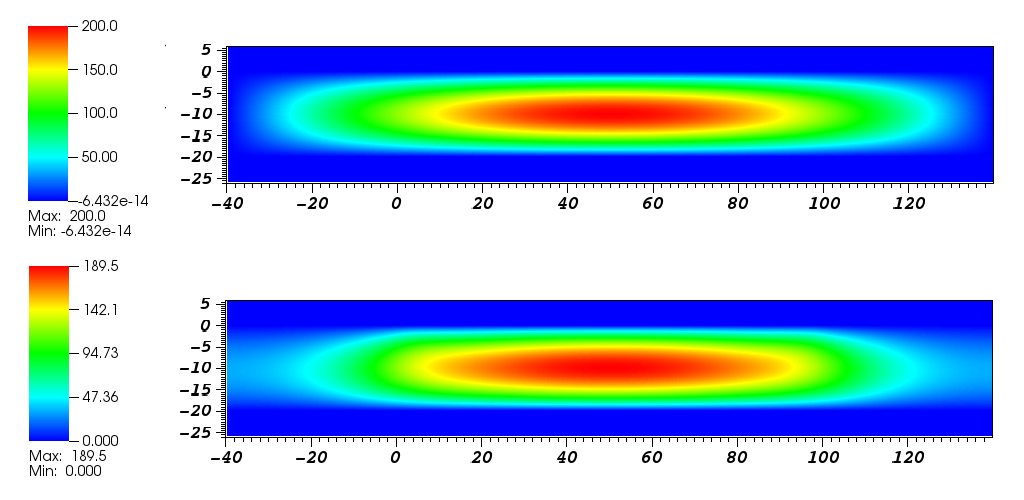
\includegraphics[width=\textwidth]{grav2D1.png}
\caption{2D density model up) reference    down) result}
\label{fig:gravity2D1}
\end{figure}


\item A 2D density properties with two maximum in corners and one minimum in the center was inverted. The result have eliminated the effects in padding area.(\ref{fig:gravity2D3}) 

\begin{verbatim}
n_cells_in_data=100
n_humbs_h= 3
n_humbs_v=1
mu=100
\end{verbatim}

\begin{figure}
\centering
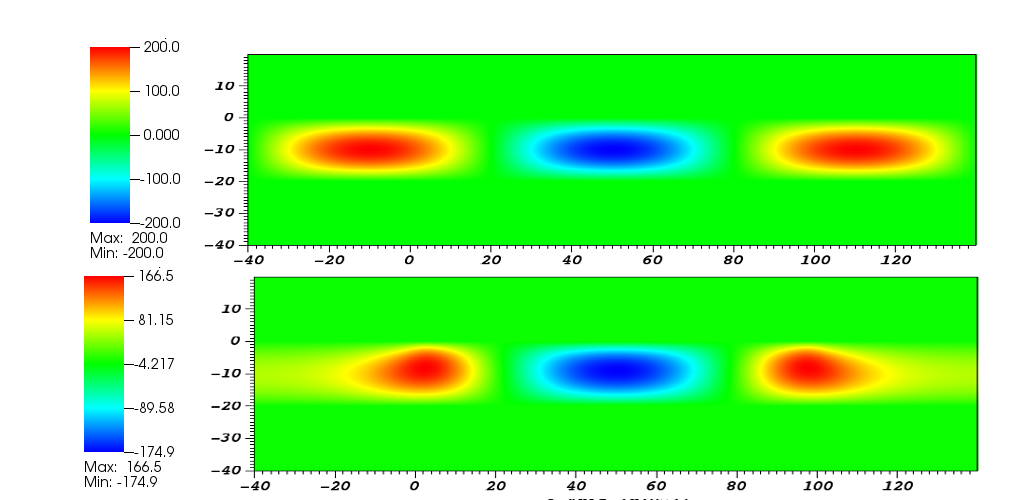
\includegraphics[width=\textwidth]{grav2D3.png}
\caption{2D density model up) reference  down) result}
\label{fig:gravity2D3}
\end{figure}

\item A 3D model with a maximum in the center was used as input data and the result after simulation in shown in the next image which determined a good distribution of density through the model in the main area.(\ref{fig:gravity3D} and \ref{fig:gravity3D1})

\begin{verbatim}
n_cells_in_data=50
n_humbs_h= 1
n_humbs_v=1
mu=10
\end{verbatim}

\begin{figure}
\centering
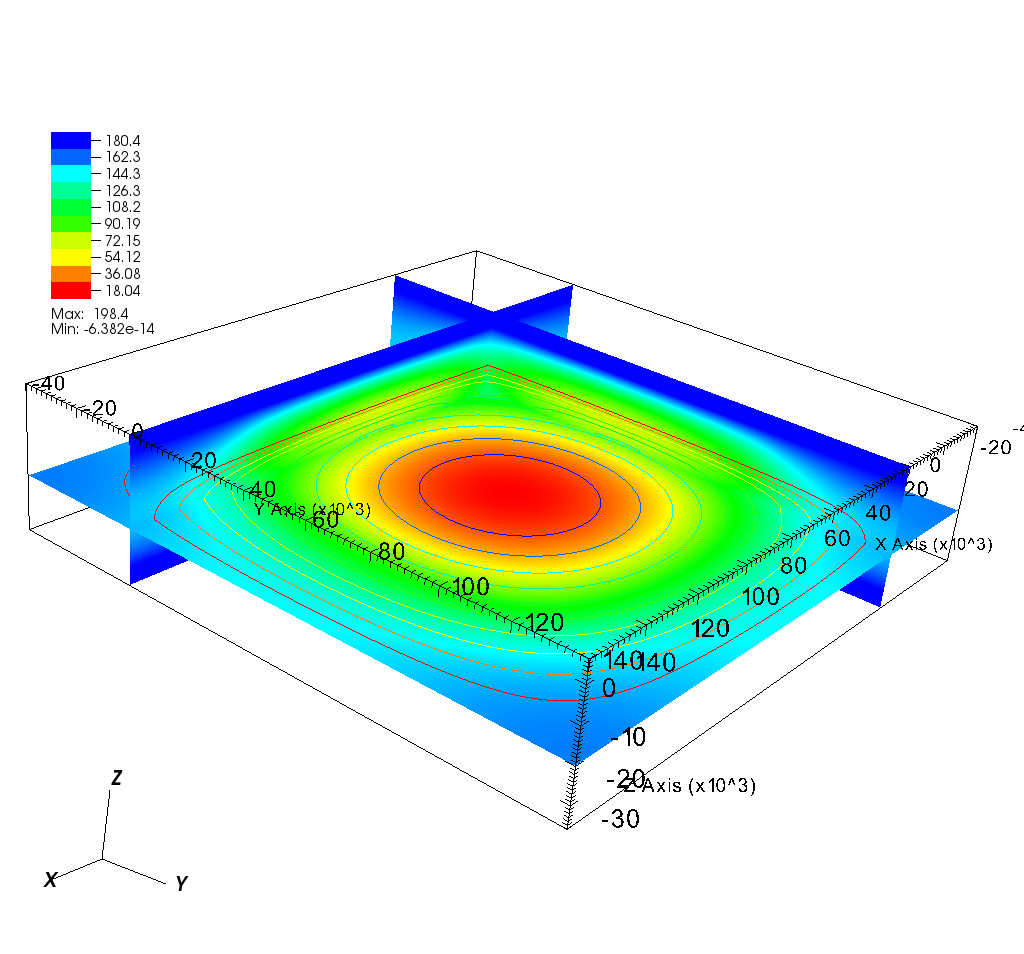
\includegraphics[width=\textwidth]{density3D-ref.png}
\caption{3D density model of reference as synthetic data}
\label{fig:gravity3D}
\end{figure}

\begin{figure}
\centering
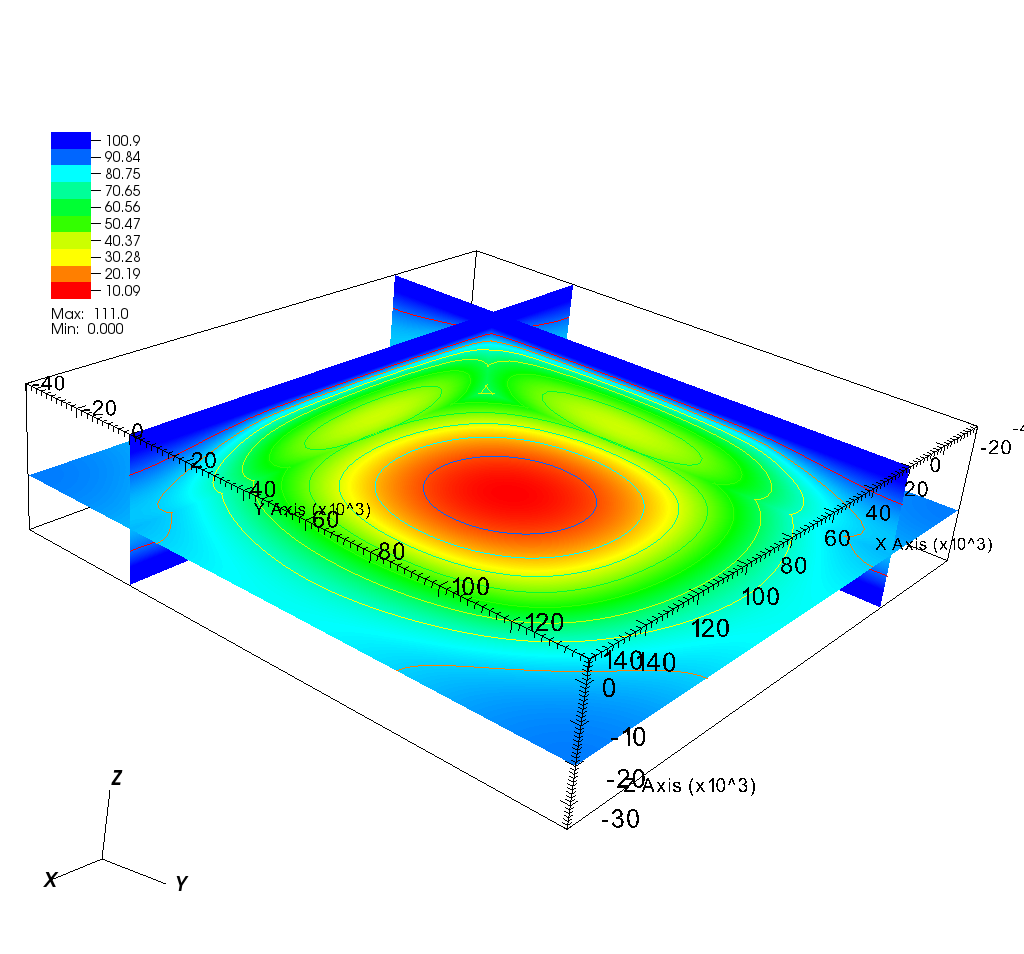
\includegraphics[width=\textwidth]{gravity3D.png}
\caption{3D density model of result}
\label{fig:gravity3D1}
\end{figure}
\end{enumerate}
